%===================================== CHAP 2 =================================

\chapter{Neuroscience context}
\label{ch:2}

Before going into the statistics and modeling, it is useful to present some context for the work. The aim of this chapter is to describe the relevant concepts from neuroscience, explain the background for the data material and provide a practical understanding. Section \ref{NandC} gives a brief description of signaling and connectivity in neural networks; the source used for this section is the book \textit{Neuroscience}, by Purves. The hallmarks for Alzheimer's disease in the brain are described in section \ref{EandA}, whose content is based on \cite{Gomez} and \cite{Witter:2011}. Section \ref{Lab} provides an outline of the lab experiments where the data that is background for this project comes from. As mentioned in the introduction, only simulated data will be used for analysis in this project. However, the methods are developed with the ultimate goal of analyzing the real data described here, which will be the object of the master project. 

\section{Concepts from neuroscience}

\subsection{Neuron and connections}\\
\label{NandC}

The basic computational unit in the brain is the nerve cell. It consists of a cell body (soma), an axon and dendrites, as illustrated in figure \ref{neuron}.
\begin{figure}[h]
    \caption{Illustration of a neuron.}
    \label{neuron}
    \centering
    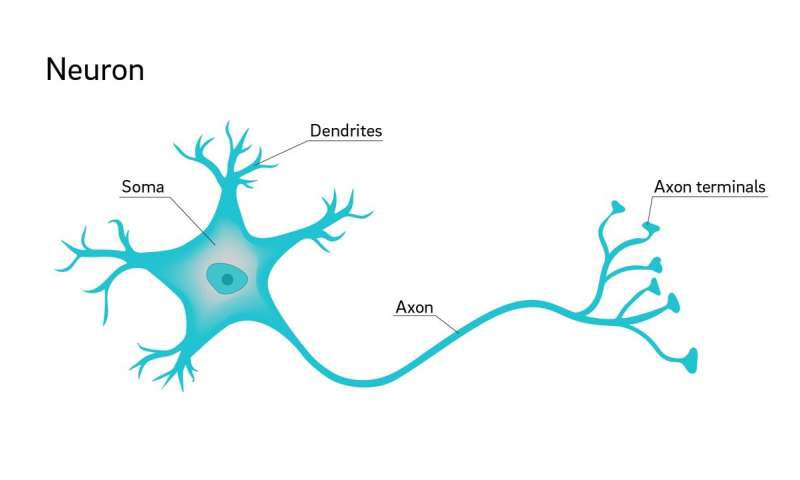
\includegraphics[scale=0.3]{Neuron.jpeg}
\end{figure} 

The computational ability of a neuron relies on its electrochemical properties. When a neuron is at rest, there is a constant potential difference across the inside and the outside of its cell membrane. This is known as the \textit{resting potential}. Ion channels embedded in the membrane allow ions to flow in and out, which can disturb the potential difference away from this equilibrium. If the voltage hits a certain threshold value, a rapid depolarization will be initiated. This phenomenon is known as an \textit{action potential}, also referred to as neuron \textit{firing} or \textit{spiking}. Whenever the threshold potential is reached, the action potential will take place no matter what. In other words there is an all-or-non property, in its typical wave form (see figure \ref{AP}). After being initiated in the soma the action potential will propagate along the axon, as illustrated to the right of figure \ref{AP}.

\begin{figure}[h]
\caption{Graphical representation of an action potential (left). Illustration of action potential propagating along axon (right).}
\label{AP}
\begin{subfigure}
\centering
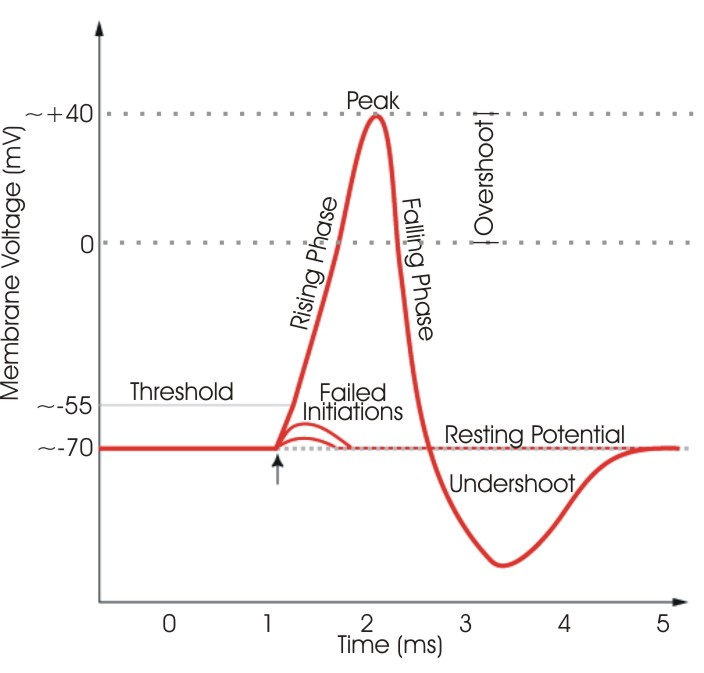
\includegraphics[scale=0.7]{AP.jpg}
\end{subfigure}
\begin{subfigure}
\centering
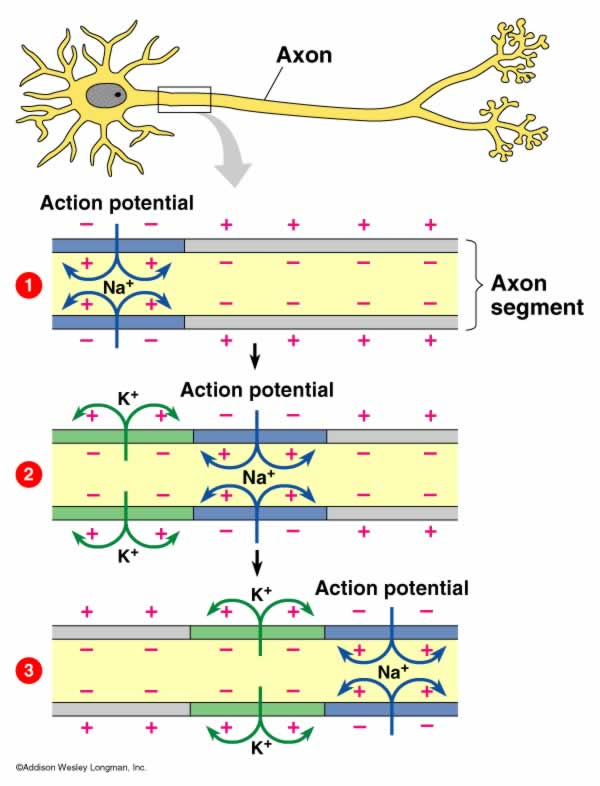
\includegraphics[scale=0.21]{Axjk4.jpg}
\end{subfigure}
\end{figure} 

The voltage increase that eventually leads to an action potential typically happens in response to stimuli from other neurons. Neurons in the brain are indeed connected to each other in a complex network. These connections are between an axon of one neuron and a dendrite of another, and are referred to as \textit{synapses}. A synapse is in practice a short gap where chemical units, called neurotransmitters, are allowed to flow from the axon of a \textit{presynaptic} neuron to the dendrite of a \textit{postsynaptic} neuron. This neurotransmitter flow, the signal, happens when the presynaptic neuron undergoes an action potential and causes an alteration in the probability with which post-synaptic ion channels open and close. This input from the pre-synaptic neuron contributes to the membrane potential (together with on average $10^4$ other neurons in the mammalian brain) which  may develop into an action potential if the threshold is reached. Sometimes the electrical signal from the presynaptic neuron increases the likelihood of an action potential to also arise in the postsynaptic neuron. In this case we say that the synapse is excitatory. This property gives rise to the possibility for a signal to propagate through the neural network, and eventually end up for example in a muscle and cause a contraction. There are also synapses that decrease the chance that the postsynaptic neuron will fire when activated. These are called inhibitory synapses.

The strength of these neural connections is not fixed, but can change over time. Strength in this sense refers to the probability that the spiking in the postsynaptic neuron will be affected by an action potential in the presynaptic neuron. A frequent activation of a synapse can strengthen the synaptic connection over time. This phenomenon is called \textit{long-term potentiation} (LTP) of a synapse. Other times activation of a synapse can weaken the connection over time. This is called \textit{long-term depression} (LTD). These changes of connections are referred to as synaptic plasticity, which is one of the basic mechanisms underlying learning and memory. \\

\subsection{Alzheimer's disease and the entorhinal cortex}
\label{EandA}

If a patient has struggles from Alzheimer's disease, the brain will eventually shrink significantly. This is due to loss of synapses and neurons, which is one of the main characteristic of the disease. Figure \ref{EC} (right) illustrates how a brain can look like after having AD for many years. Exactly what causes these losses is still not known, but it is assumed that the accumulation of some protein types called amyloid plaques and neurofirbillary tangles are involved. Another hallmark of AD is impaired neural activity, which may be related to dysfunctional plasticity mechanisms (\cite{Zott}). Therefore, it is interesting to investigate whether healthy brains and brains with AD can be distinguished due to their synaptic plasticity properties.

\begin{figure}[h]
    \caption{(Left) Illustration of brain showing location of the Entorhinal cortex. (Right) Visual comparison of healthy brain and brain with Alzheimer's disease.}
    \label{EC}
    \centering
    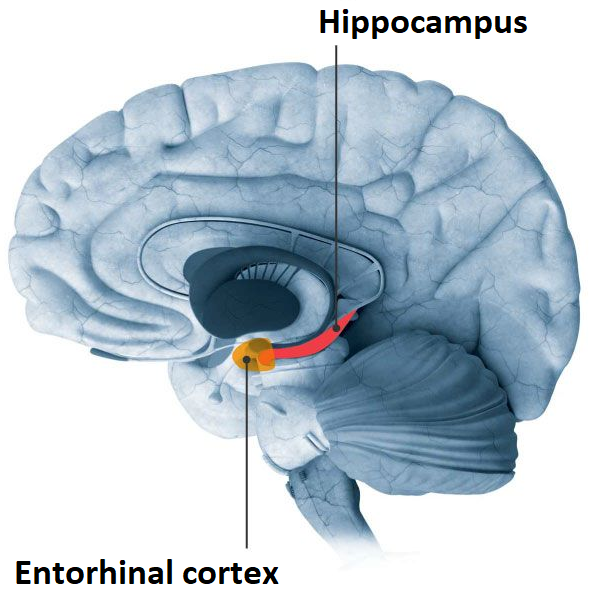
\includegraphics[scale=0.35]{Entorhinal_cortex2.png}
    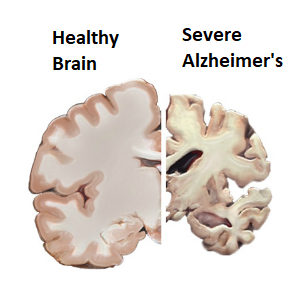
\includegraphics[scale=0.8]{fig/Alzheimers_picture.png}    
    \label{brain}
\end{figure} 

One target area in the brain for Alzheimer's research is the \textit{entorhinal cortex}, which is associated with the earliest indications of AD. The entorhinal cortex is a brain region that is phylogenetically conserved across species, so research on how AD develops in rat's entorhinal cortex can give insights for humans as well. It is found in the medial temporal lobe and functions as a gateway between the neocortex and the hippocampus, which is known to be involved in declarative memory and learning. The position  of the entorhinal cortex in the brain is shown in figure \ref{EC} (left). The entorhinal cortex is commonly subdivided into six layers, I-VI. Cells in layer II of the entorhinal cortex are shown to be affected in the initial stages of AD. Therefore layer II neurons are object of the experiments we will get the data from to study how AD affects the synaptic plasticity.




\section{Data material}

\label{Lab}\\
The data material that is the background for this project is electric potential recordings from in-vitro cultured neural networks from rat brains. Rats do not get Alzheimer's naturally, so AD rats are designed with a genetic mutation that gives rise to amyloid plaque accumulation in their brains. It was shown that at an age of 8 months, mice with this mutation have learning impairments and behavioural differences from healthy mice (\cite{Radde}). 

In short, tissue from layer II of the entorhinal cortex is gathered by microdissection from rat brains (\cite{Katrine}), and the embedded neurons are dissociated from their biological substrate to be plated into a dish. Next the seeded neurons are cultured in a mean, which allows them to survive and grow new connections. Once the network is mature, microelectrode arrays, a sheet of equally spaced needle electrodes, are then used to record the electrical activity of the neurons. Preferably each electrode should measure the activity of one neuron only. However, the recordings are extracellular, which means that the electrodes might pick up signals from several neurons. Therefore, a spike sorting procedure is performed to assign the recorded action potentials to single neurons. 

It is the time points for the action potentials that are of interest, and not the actual voltage values. Hence, the relevant data material is a sequence of recorded time points for the action potentials for each neuron, in the time interval $[0,K]$. This can be written as, 
\begin{equation}
\label{eq:AP}
    \{\{a_i\}\}_{i=1}^{N} = \{a_{i1}, a_{i2}, ...\}_{i=1}^{N} \quad a_{ix} \in [0,K]
\end{equation}

where $a_{ix}$ is the recorded time for the $x'th$ action potential of neuron $i$, $a_{ix-1} < a_{ix}$, and $i=1,2,...,N$ labels the neurons. Such a sequence of time stamps for a single firing neuron is called a \textit{spike train}.\\



%One electrode can measure the electrical activity of one neuron over time interval $[0,K]$. When a neuron undergoes an action potential, this will appear as a peak in these recordings.



\cleardoublepage